\documentclass[svgnames,11pt]{beamer}
\input{/home/tof/Documents/Cozy/latex-include/preambule_commun.tex}
\input{/home/tof/Documents/Cozy/latex-include/preambule_beamer.tex}
%\usepackage{pgfpages} \setbeameroption{show notes on second screen=left}
\author[]{Christophe Viroulaud}
\title{Architecture d'un ordinateur}
\date{\framebox{\textbf{ArchMat 01}}}
%\logo{}
\institute{Première - NSI}

\begin{document}
\begin{frame}
\titlepage
\end{frame}
\begin{frame}
    \frametitle{}

Ordinateur de bureau, ordinateur portable, smartphone, tablette, montre connectée, voiture autonome\dots toutes ces machines ont envahi notre quotidien. Les usages sont variés, cependant, certains principes généraux semblent exister.
\begin{center}
    \begin{tabular}{ccc}
        \includegraphics[width=3cm]{ressources/smartphone.jpeg}&
        \includegraphics[width=3cm]{ressources/frigo.png}&
        \includegraphics[width=3cm]{ressources/voiture.jpg}
    \end{tabular}
\end{center}
\framebox{Peut-on décrire une architecture commune à toutes ces machines?}

\end{frame}
\section{Première approche: à chaque composant son rôle}
\subsection{CPU}
\begin{frame}
    \frametitle{CPU}

    \begin{center}
    \centering
    \includegraphics[width=5cm]{ressources/processeur.jpg}
    \captionof{figure}{Control Processing Unit (CPU)}
    \label{IMG}
    \end{center}
\begin{aretenir}[]
Le microprocesseur (ou processeur) effectue les calculs. On le caractérise souvent par le nombre d'opérations réalisables par seconde: la \emph{fréquence}.
\end{aretenir}
\end{frame}
\begin{frame}
    \frametitle{Loi de Moore}

    \begin{center}
    \centering
    \includegraphics[width=8cm]{ressources/Loi_de_Moore.png}
    \captionof{figure}{Loi de Moore}
    \label{IMG}
    \end{center}

\note[item]{loi empirique; nd de transistors doublent tous les 2 ans et donc puissance de calcul augmente}
\note[item]{loi vérifiée jusqu'en 2004; bute sur effet thermique $\rightarrow$ multiprocesseurs donc loi toujours valable}
\end{frame}
\subsection{Mémoires}
\begin{frame}
    \frametitle{Mémoires}

    \begin{center}
    \centering
    \includegraphics[width=5cm]{ressources/barrette.jpg}
    \captionof{figure}{Mémoire vive (Random Access Memory)}
    \label{IMG}
    \end{center}
\begin{aretenir}[]
La mémoire contient les \textbf{données} et les \textbf{instructions} (programme) que le processeur va utiliser.
\end{aretenir}
\note{deux adresses choisies aléatoirement ont le même temps d'accès}
\end{frame}
\begin{frame}
    \frametitle{Différence de vitesses}

    \begin{center}
        Cadence processeur: $3GHz \rightarrow 3×10^9$ opérations par seconde
    \end{center}
    \begin{tabular}{|*{3}{c|}}
        \hline 
        Type de mémoire & Temps d'accès & Accès par seconde \\ 
        \hline 
        registres & 1ns &$\simeq 10^9$ \\ 
        \hline 
        mémoire cache & 3ns &$\simeq 10^8$ \\
        \hline
        mémoire vive & 50ns &$\simeq 10^7$ \\
        \hline
        disques durs & 10ms & $\simeq 10^2$ \\
        \hline
        DVD & 140ms&$\simeq 10^1$ \\
        \hline
        \end{tabular} 

\end{frame}
\begin{frame}
    \frametitle{}

    \begin{center}
        {\Large Il faut optimiser le temps d'utilisation du processeur.}
    \end{center}

\end{frame}
\begin{frame}
    \frametitle{Plusieurs mémoires}

    \begin{center}
    \centering
    \includegraphics[width=8cm]{ressources/memoires.jpg}
    \captionof{figure}{Plus la mémoire est rapide plus elle est proche du CPU.}
    \end{center}
\note[item]{SRAM = Static RAM; plus rapides mais plus chères = mémoire cache}
\note[item]{DRAM = Dynamic RAM; moins chères mais moins rapides = mémoire vive barrette}
\note[item]{cache = L1, L2, L3 $\rightarrow$ à regarder quand on achète un PC}
\end{frame}
\subsection{Entrées - sorties}
\begin{frame}
    \frametitle{Entrées}

    Pour alimenter la machine (en données et instructions) il faut une \emph{interface} d'entrée.
\begin{center}
    \begin{tabular}{ccc}
        \includegraphics[width=3cm]{ressources/clavier.jpg}&
        \includegraphics[width=3cm]{ressources/souris.jpg}&
        \includegraphics[width=3cm]{ressources/webcam.jpg}\\
    \end{tabular}
\end{center}

\end{frame}
\begin{frame}
    \frametitle{Sorties}

Pour que l'utilisateur récupère les résultats, il faut une \emph{interface} de sortie.
\begin{center}
    \begin{tabular}{ccc}
        \includegraphics[width=3cm]{ressources/ecran.jpg}&
        \includegraphics[width=3cm]{ressources/imprimante.jpg}&
        \includegraphics[width=3cm]{ressources/enceinte.jpg}\\
    \end{tabular}
\end{center}

\end{frame}
\section{Le modèle de von Neumann}
\subsection{Approche détaillée}
\begin{frame}
    \frametitle{Le modèle de von Neumann}
\begin{center}
    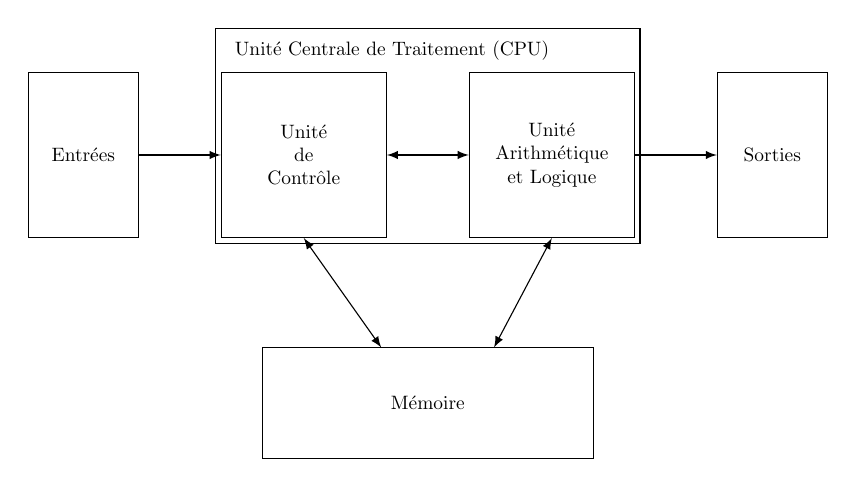
\begin{tikzpicture}[every text node part/.style={align=center},scale=0.7, transform shape]
        \draw (-0.1,-0.1)--(7.6,-0.1)--(7.6,3.8)--(-0.1,3.8)--cycle;
        \node at (3.1,3.4) {Unité Centrale de Traitement (CPU)};
        \node[draw,minimum width=3cm,minimum height=3cm] (uc) at (1.5,1.5){Unité \\ de \\ Contrôle};
        \node[draw,minimum width=3cm,minimum height=3cm] (ual) at (6,1.5){Unité \\ Arithmétique \\ et Logique};

        \node[draw,minimum width=6cm,minimum height=2cm] (mem) at (3.75,-3){Mémoire};
        \node[draw,minimum width=2cm,minimum height=3cm] (i) at (-2.5,1.5){Entrées};
        \node[draw,minimum width=2cm,minimum height=3cm] (o) at (10,1.5){Sorties};
        \draw[<->,>=latex] (ual.south) -- (mem.40);
        \draw[<->,>=latex] (uc.east) -- (ual.west);
        \draw[->,>=latex] (i.east) -- (uc.west);
        \draw[<->,>=latex] (uc.south) -- (mem.130);
        \draw[->,>=latex] (ual.east) -- (o.west);

    \end{tikzpicture}
\end{center}

\note[item]{le modèle présenté en 2 est une approche simplifiée du modèle de von Neumann}
\note[item]{Que reconnait-on?}
\end{frame}
\begin{frame}
    \frametitle{}

    \begin{itemize}
        \item<1-> CPU:
        \begin{itemize}
            \item Unité de Contrôle:
            \begin{itemize}
                \item décode les instructions,
                \item commande leur exécution par l'UAL.
            \end{itemize}
            \item Unité Arithmétique et Logique: effectue les calculs.
        \end{itemize}
        \item<2-> Mémoire: stocke les données et les instructions.
        \item<3->Entrées/Sorties
    \end{itemize}
\end{frame}

\section{Un modèle hérité}
\begin{frame}
    \frametitle{Un modèle hérité}

\begin{aretenir}[]
    Von Neumann a présenté son modèle en 1945. Son concept est toujours en vigueur dans les ordinateurs actuels.

\end{aretenir}
\end{frame}
\subsection{Automatisation}
\begin{frame}
    \frametitle{Automatisation}

Les Hommes ont utilisé la mécanique (XIX°) puis l'électronique (XX°) pour automatiser les tâches, les calculs.

\end{frame}
\begin{frame}
    \frametitle{}

    \begin{center}
    \centering
    \includegraphics[width=6cm]{ressources/babbage.jpg}
    \end{center}
\begin{aretenir}[1834-1836]
    Charles Babbage imagine la machine analytique: une machine à calculer programmable. Ada Lovelace conçoit le premier programme informatique.
\end{aretenir}
\end{frame}
\begin{frame}
    \frametitle{}

    \begin{center}
    \centering
    \includegraphics[width=6cm]{ressources/zuse.jpg}
    \end{center}
\begin{aretenir}[1938-1941]
    L’allemand Konrad Zuse achève le Z1 en 1938, un ordinateur mécanique en binaire, puis le Z3 en 1941: il réalisait 3-4 additions par seconde.
\end{aretenir}
\end{frame}
\begin{frame}
    \frametitle{}

    \begin{center}
    \centering
    \includegraphics[width=4cm]{ressources/atanasoff.jpg}
    \end{center}
\begin{aretenir}[1942]
    Il construit la première machine électronique sans l'achever complètement. Ses idées seront reprises par Mauchly et Eckert.
\end{aretenir}
\end{frame}
\begin{frame}
    \frametitle{}

    \begin{center}
    \centering
    \includegraphics[width=6cm]{ressources/eniac.jpg}
    \end{center}
\begin{aretenir}[1945]
    Mauchly et Eckert conçoivent le premier ordinateur entièrement électronique: ENIAC (Electronic Numerical Integrator And Computer)
\end{aretenir}
\note[item]{on peut également citer le Colossus en 1943 en Grande-Bretagne}
\note[item]{objectifs militaires: effectuer des calculs balistiques}
\end{frame}
\begin{frame}
    \frametitle{}

\begin{itemize}
    \item Ces calculateurs électroniques ne pouvaient exécuter qu'un seul programme à la fois.
    \item Il fallait reconfigurer la machine pour remplir une autre tâche.
\end{itemize}
\begin{center}
\centering
\includegraphics[width=6cm]{ressources/configeniac.jpg}
\captionof{figure}{Opératrices configurant l'ENIAC}
\label{IMG}
\end{center}
\end{frame}
\begin{frame}
    \frametitle{}

    \begin{aretenir}[]
    L'idée principale de John von Neumann est de considérer un programme comme une donnée. Il sera stocké dans la mémoire.
    \end{aretenir}
    \begin{center}
        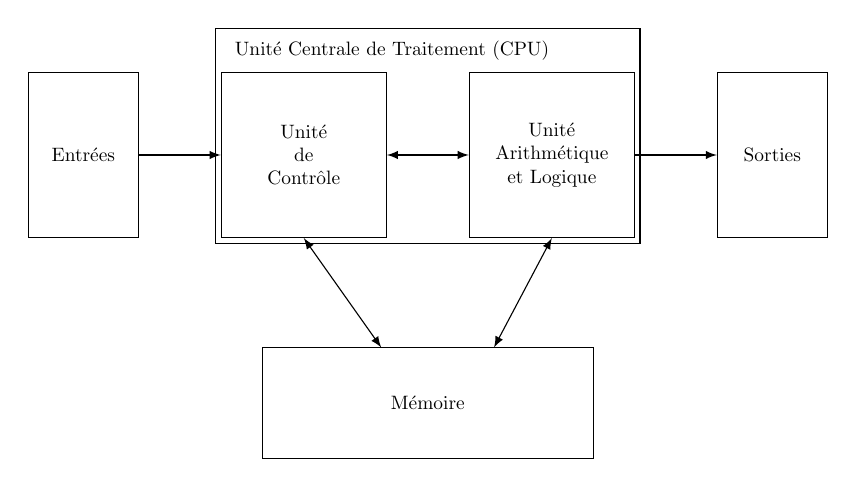
\begin{tikzpicture}[every text node part/.style={align=center},scale=0.7, transform shape]
            \draw (-0.1,-0.1)--(7.6,-0.1)--(7.6,3.8)--(-0.1,3.8)--cycle;
            \node at (3.1,3.4) {Unité Centrale de Traitement (CPU)};
            \node[draw,minimum width=3cm,minimum height=3cm] (uc) at (1.5,1.5){Unité \\ de \\ Contrôle};
            \node[draw,minimum width=3cm,minimum height=3cm] (ual) at (6,1.5){Unité \\ Arithmétique \\ et Logique};
    
            \node[draw,minimum width=6cm,minimum height=2cm] (mem) at (3.75,-3){Mémoire};
            \node[draw,minimum width=2cm,minimum height=3cm] (i) at (-2.5,1.5){Entrées};
            \node[draw,minimum width=2cm,minimum height=3cm] (o) at (10,1.5){Sorties};
            \draw[<->,>=latex] (ual.south) -- (mem.40);
            \draw[<->,>=latex] (uc.east) -- (ual.west);
            \draw[->,>=latex] (i.east) -- (uc.west);
            \draw[<->,>=latex] (uc.south) -- (mem.130);
            \draw[->,>=latex] (ual.east) -- (o.west);
    
        \end{tikzpicture}
    \end{center}
\end{frame}
\begin{frame}
    \frametitle{}

    \begin{center}
    \centering
    \includegraphics[width=6cm]{ressources/edvac.jpg}
    \captionof{figure}{EDVAC (Electronic Discrete Variable Automatic Computer)}
    \label{IMG}
    \end{center}
\begin{aretenir}[1945]
Von Neumann accepte un poste de consultant dans le projet EDVAC, successeur de l'ENIAC.
\end{aretenir}
\note{Le rapport EDVAC circula largement et eut une influence notable sur bon nombre de travaux ultérieurs.}
\end{frame}
\subsection{Modèle universel}
\begin{frame}
    \frametitle{Modèle universel}
\begin{center}
    \includegraphics[width=8cm]{ressources/cartemere.png}
\end{center}
\includegraphics[width=3cm]{ressources/inside.jpg}

\end{frame}
\begin{frame}
    \frametitle{}
\begin{center}
\centering
\includegraphics[width=4cm]{ressources/voiture.jpg}
\end{center}
    \begin{center}
        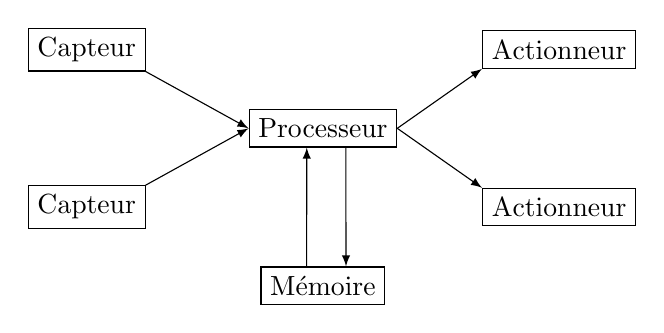
\begin{tikzpicture}
            \node[draw] (p)at(0,0) {Processeur};
            \node[draw] (m)at(0,-2) {Mémoire};
            \node[draw] (c1)at(-3,1) {Capteur};
            \node[draw] (c2)at(-3,-1) {Capteur};
            \node[draw] (a1)at(3,1) {Actionneur};
            \node[draw] (a2)at(3,-1) {Actionneur};
            \draw[->,>=latex] (p.-40) -- (m.40);
            \draw[->,>=latex] (m.130) -- (p.-130);
            \draw[->,>=latex] (c1.south east) -- (p.west);
            \draw[->,>=latex] (c2.north east) -- (p.west);
            \draw[->,>=latex] (p.east) -- (a1.south west);
            \draw[->,>=latex] (p.east) -- (a2.north west);

        \end{tikzpicture}
        \captionof{figure}{Système embarqué d'une voiture autonome}
        \label{sie}
    \end{center}

\end{frame}
\subsection{Évolutions du modèle}
\begin{frame}
    \frametitle{Évolutions du modèle}

\begin{itemize}
    \item<1-> Les entrées-sorties, initialement commandées par l’unité centrale, sont depuis le début des années 1960 sous le contrôle de processeurs autonomes.
    \item<2-> Les ordinateurs comportent maintenant des processeurs multiples.
    \item<3-> Il existe des processeurs spécialisés (carte graphique).
    \item<4-> La carte-mère relie les différentes unités du modèle.
    \item<5-> La mémoire vive s'efface à l'extinction de la machine.
    \item<6-> La mémoire ROM (Read Only Memory) est persistante. Elle contient la séquence de démarrage.
\end{itemize}

\end{frame}
\begin{frame}
    \frametitle{Bibliographie}
    {\small
    \begin{itemize}
        \item \url{https://interstices.info/le-modele-darchitecture-de-von-neumann/}
        \item \url{https://fr.wikipedia.org/wiki/Architecture_de_von_Neumann}
        \item \url{https://www.cours.jlrichter.fr/}
        \item NSI 1° - éditions Ellipses
    \end{itemize}
    }
\end{frame}
\end{document}